\section{Correctness Changes the Usable Execution Path}
\label{sec:admissibility}
% Evidence: M4-MICRO, RTX-MICRO, B570-FAST/SERIAL.
\begin{figure*}[t]
\centering
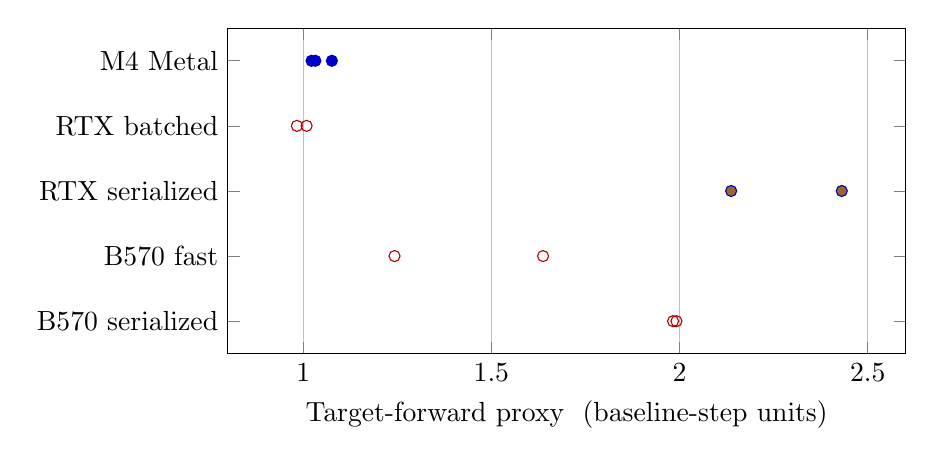
\begin{tikzpicture}
\begin{axis}[width=.84\textwidth,height=2.25in,xmin=.8,xmax=2.6,ymin=-.5,ymax=4.5,y dir=reverse,ytick={0,1,2,3,4},yticklabels={M4 Metal,RTX batched,RTX serialized,B570 fast,B570 serialized},xlabel={Target-forward proxy $\vTwo$ (baseline-step units)},xtick={1,1.5,2,2.5},xmajorgrids,axis on top]
\addplot[black,dashed,forget plot] coordinates {(1,-.5)(1,4.5)};
% Point pairs/triples at distinct contexts; not uncertainty intervals.
\addplot+[only marks,mark=*,color=blue!70!black] coordinates {(1.0221818546851145,0) (1.0761256101952625,0) (1.0322635228699184,0)};
\addplot+[only marks,mark=o,color=red!70!black] coordinates {(1.0090304299186035,1) (0.9831479829424705,1)};
\addplot+[only marks,mark=*,color=blue!70!black] coordinates {(2.43099575218514,2) (2.137011311768208,2)};
\addplot+[only marks,mark=o,color=red!70!black] coordinates {(1.2426,3) (1.6373,3)};
\addplot+[only marks,mark=o,color=red!70!black] coordinates {(1.982667717765499,4) (1.991706889255509,4)};

\end{axis}
\end{tikzpicture}
\caption{How does correctness change usable verification? Filled marks: paths exact on the frozen reported workloads; open marks: correctness-blocked paths (including B570 serialized). Each mark is one context cell; nearby cells can overlap. M4 contexts: 512/2048/8192; RTX 5070 Ti Laptop depths: 0/256; B570 contexts: 512/2048. Contexts, runtimes, and controls differ: this is not a hardware ranking. The plotted proxy is not complete $\rtarget$.}
\label{fig:verification}
\end{figure*}

% Evidence: M4-MICRO, RTX-MICRO, B570-FAST/SERIAL.
\begin{table}[t]
\caption{Verification/admissibility mechanism. Proxy ranges span measured contexts, not confidence intervals. Full target-round $\rtarget$ is not exposed by these microbenchmarks.}
\label{tab:mechanism}
\centering
\begin{tabular}{>{\raggedright\arraybackslash}p{0.85in}>{\raggedright\arraybackslash}p{0.66in}>{\raggedright\arraybackslash}p{1.23in}}
\toprule
Path & $\vTwo$ & Qualification \\
\midrule
M4 Metal & 1.02--1.08 & Frozen workloads exact \\
RTX batched & 0.98--1.01 & Correctness-blocked \\
RTX serial & 2.14--2.43 & Exact secondary control \\
B570 fast & 1.24--1.64 & 45/90 exact; diagnostic \\
B570 serial & 1.98--1.99 & 60/90 exact; diagnostic \\
\bottomrule
\end{tabular}
\end{table}

\subsection{Cheap physical batching is not sufficient}
The final M4 Metal path combines exact frozen-workload outputs with a target-forward proxy near one baseline step. Across its tested contexts, $\vTwo$ is approximately 1.02--1.08. This is a batching opportunity, not a complete round decomposition, and does not by itself explain whether a workload is profitable.

On RTX 5070 Ti Laptop, the batched CUDA target also has near-one-step two-token forward cost: $\vTwo=\RTXrawZero$ and $\RTXrawDepth$ at the two measured depths. The intended fast HumanEval execution nevertheless fails the frozen token-equivalence gate. Its timings cannot support an admissible optimization claim. The serialized control changes the micro-batch to one and raises the measured proxy to $\RTXserZero$ and $\RTXserDepth$; the full frozen exact-control workload passes. Figure~\ref{fig:verification} therefore relates a physical opportunity to its empirically qualified status, rather than ranking GPUs.

\subsection{A bounded numerical divergence}
The frozen CUDA reproducer repeats the HumanEval/106 divergence in three of three runs at the same captured location. Sequential and serialized execution select token 2790, whereas batched execution selects 2629. A separate same-commit diagnostic build captures the corresponding score-margin change from $+0.080948$ to $-0.126457$. That numerical instrumentation does not replace the original formal binary or its measurements.

The evidence supports stable batch-shape-dependent greedy argmax divergence in this llama.cpp/CUDA/Q8\_0 configuration. It does not identify a universal CUDA failure or a specific responsible kernel. Floating-point and batch-dependent output differences are established research topics \citep{numerics,llm42}; the systems consequence here is that the cheap path is removed from the set admitted by the study's contract.

\subsection{Serialization does not establish exactness}
B570 provides a complementary boundary. Its formal v2 correctness gate fails, so the preregistered stop rule prevents a formal verification/performance claim from that execution. Later fast-path diagnostics yield \BFastExact/90\ exact pairs. The unique serialized fallback improves this to \BExact/90, with \BExactPrompts/30\ wholly exact prompts, but still fails workload-global equality. Its $\vTwo$ is approximately \BvShort--\BvLong\ and remains diagnostic.

A smaller serialized probe had passed before the full workload exposed mismatches. Passing such a gate is evidence for its tested scope, not proof of broader correctness. We therefore use ``serialized $\vTwo$'' or ``V2\_serialized'' for this B570 path. An execution property must not be renamed as an exactness guarantee.
